\documentclass[12pt,oneside]{report}
%%%%%%%%%%%%%%%%%%%%%%%%%%%%%%%%%%%%%%%%%%%%%%%%%%%%%%%%%%%%%%%%%%%%%%%%%%%%%%%
\input{preambule_2024}
%%%%%%%%%%%%%%%%%%%%%%%%%%%%%%%%%%%%%%%%%%%%%%%%%%%%%%%%%%%%%%%%%%%%%%%%%%%%%%%
\portrait
%\paysage
%\usepackage{cclicenses}
%%%%%%%%%%%%%%%%%%%%%%%%%%%%%%%%%%%%%%%%%%%%%%%%%%%%%%%%%%%%%%%%%%%%%%%%%%%%%%%
%%%%%%%%À modifier !!!!!!!!!!!!!!!!
\newcommand{\classe}{\LaTeX{} }
\newcommand{\titredoc}{\fontfamily{pzc}
\bfseries\fontsize{30}{20}\selectfont{Bar charts with TikZ}%\par
}
\newcommand{\auteurs}{\LaTeX{}}

%%%%%%%%%%%%%%%%%%%%%%%%%%%%%%%%%%%%%%%%%%%%%%%%%%%%%%%%%%%%%%%%%%%%%%%%%%%%%%%
\fancyhf{}
\rhead{ \textcolor{orange!90}{\bsc{\large \classe}}}
\lhead{}
\rfoot{\textcolor{blue}{Licence : \ccbyncsaeu}}

\lfoot{ \textcolor{blue}{\auteurs}}
\cfoot{\thepage / \pageref{LastPage}}
\renewcommand \headrulewidth{0pt}
\renewcommand {\footrule}{{\color{orange!70}\rule{\textwidth}{0.9pt}}}
\pagestyle{fancy}
%\tikzset{domaine/.style 2 args={domain=#1:#2}}

%%%%%%%%%%%%%%%%%%%%%%%%%%%%%%%%%%%%%%%%%%%%%%%%%%%%%%%%%%%%
\usepackage[linesnumbered,french]{algorithm2e}
%%%%%%%%%%%%%%%%%%%%%%%%%%%%%%%%%%%%%%%%%%%%%%%%%%%%%%%%%%%%
\newcommand{\cadrevide}[1]{
\begin{Cadre}
\begin{minipage}{\linewidth}
\vspace{#1}
\end{minipage}
\end{Cadre}}
%%%%%%%%%%%%%%%%%%%%%%%%%%%%%%%%%%%%%%%%%%%%%%%%%%%%%%%%%%%%
\begin{document}
\selectlanguage{english}

\begin{Cadre}
\vspace*{1em}
\begin{tabular}{m{0.15\linewidth}M{0.63\linewidth}R{0.15\linewidth}}

\includegraphics[width=\linewidth]{logo_augustin_thierry}
&
\textcolor{blue}{
\titredoc
}
&

\includegraphics[width=0.7\linewidth]{logo_acad}
\end{tabular}
\vspace*{0.2em}
\end{Cadre}

%%%%%%%%%%%%%%%%%%%%%%%%%%%%%%%%%%%%%%%%%%%%%%%%%%%%%%%%%%%%
\begin{spacing}{1.2}
%%%%%%%%%%%%%%%%%%%%%%%%%%%%%%%%%%%%%%%%%%%%%%%%%%%%%%%%%%%%

\begin{center}
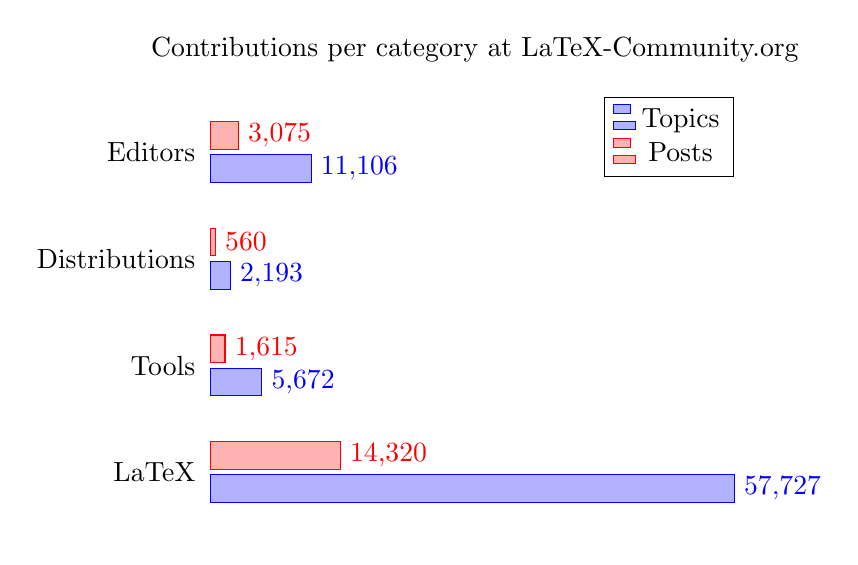
\begin{tikzpicture}
  \begin{axis}[title  = Contributions per category
                          at LaTeX-Community.org,
    xbar,
    y axis line style = { opacity = 0 },
    axis x line       = none,
    tickwidth         = 0pt,
    enlarge y limits  = 0.2,
    enlarge x limits  = 0.02,
    symbolic y coords = {LaTeX, Tools, Distributions, Editors},
    nodes near coords,
  ]
  \addplot coordinates { (57727,LaTeX)         (5672,Tools)
                         (2193,Distributions)  (11106,Editors) };
  \addplot coordinates { (14320,LaTeX)         (1615,Tools)
                         (560,Distributions)   (3075,Editors)  };
  \legend{Topics, Posts}
  \end{axis}
\end{tikzpicture}
\end{center}

%%%%%%%%%%%%%%%%%%%%%%%%%%%%%%%%%%%%%%%%%%%%%%%%%%%%%%%%%%%%%%%

\begin{center}
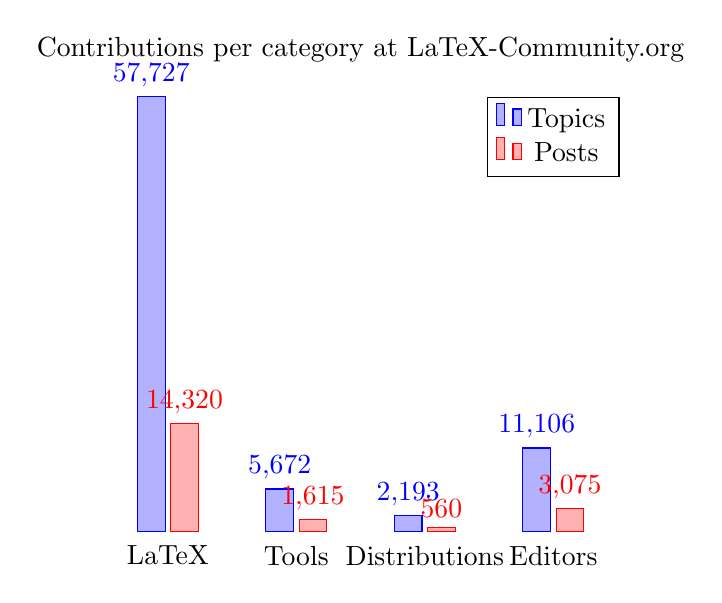
\begin{tikzpicture}
  \begin{axis}[title  = Contributions per category
                          at LaTeX-Community.org,
    ybar,
    x axis line style = { opacity = 0 },
    axis y line       = none,
    tickwidth         = 0pt,
    enlarge x limits  = 0.2,
    enlarge y limits  = 0.02,
    symbolic x coords = {LaTeX, Tools, Distributions, Editors},
    nodes near coords,
  ]
  \addplot coordinates { (LaTeX,57727)         (Tools,5672)
                         (Distributions,2193)  (Editors,11106) };
  \addplot coordinates { (LaTeX,14320)         (Tools,1615)
                         (Distributions,560)   (Editors,3075)  };
  \legend{Topics, Posts}
  \end{axis}
\end{tikzpicture}
\end{center}

%%%%%%%%%%%%%%%%%%%%%%%%%%%%%%%%%%%%%%%%%%%%%%%%%%%%%%%%%%%%%%%

\begin{center}
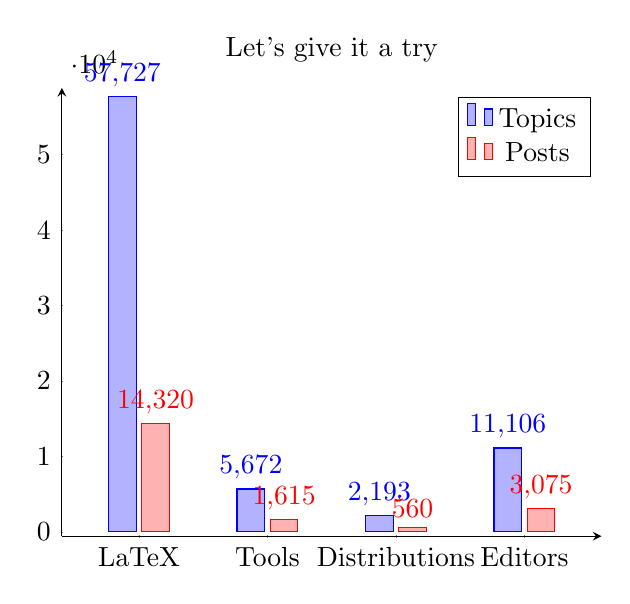
\begin{tikzpicture}
  \begin{axis}[title  = Let's give it a try,
    ybar,
    axis lines  		= left,
    tickwidth         = 1pt,
    enlarge x limits  = 0.2,
    enlarge y limits  = 0.02,
    symbolic x coords = {LaTeX, Tools, Distributions, Editors},
    nodes near coords,
  ]
  \addplot coordinates { (LaTeX,57727)         (Tools,5672)
                         (Distributions,2193)  (Editors,11106) };
  \addplot coordinates { (LaTeX,14320)         (Tools,1615)
                         (Distributions,560)   (Editors,3075)  };
  \legend{Topics, Posts}
  \end{axis}
\end{tikzpicture}
\end{center}

%%%%%%%%%%%%%%%%%%%%%%%%%%%%%%%%%%%%%%%%%%%%%%%%%%%%%%%%%%%%%%%

\begin{center}
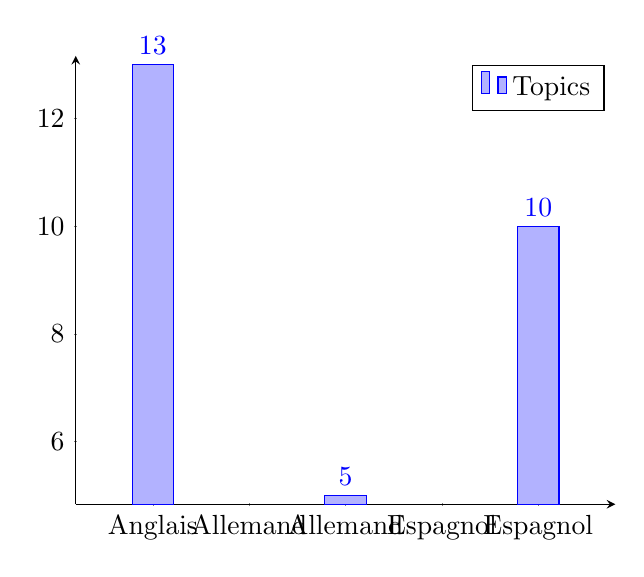
\begin{tikzpicture}
  \begin{axis}[title=,
    ybar, ,bar width=15pt,
    axis lines  		= left,
    tickwidth         = 1pt,
    enlarge x limits  = 0.2,
    enlarge y limits  = 0.02,
    symbolic x coords = {Anglais, Allemand, Espagnol},
    nodes near coords,
  ]
  \addplot coordinates { (Anglais, 13) (Allemand, 5) (Espagnol, 10)};
  \legend{Topics, Posts}
  \end{axis}
\end{tikzpicture}
\end{center}

%%%%%%%%%%%%%%%%%%%%%%%%%%%%%%%%%%%%%%%%%%%%%%%%%%%%%

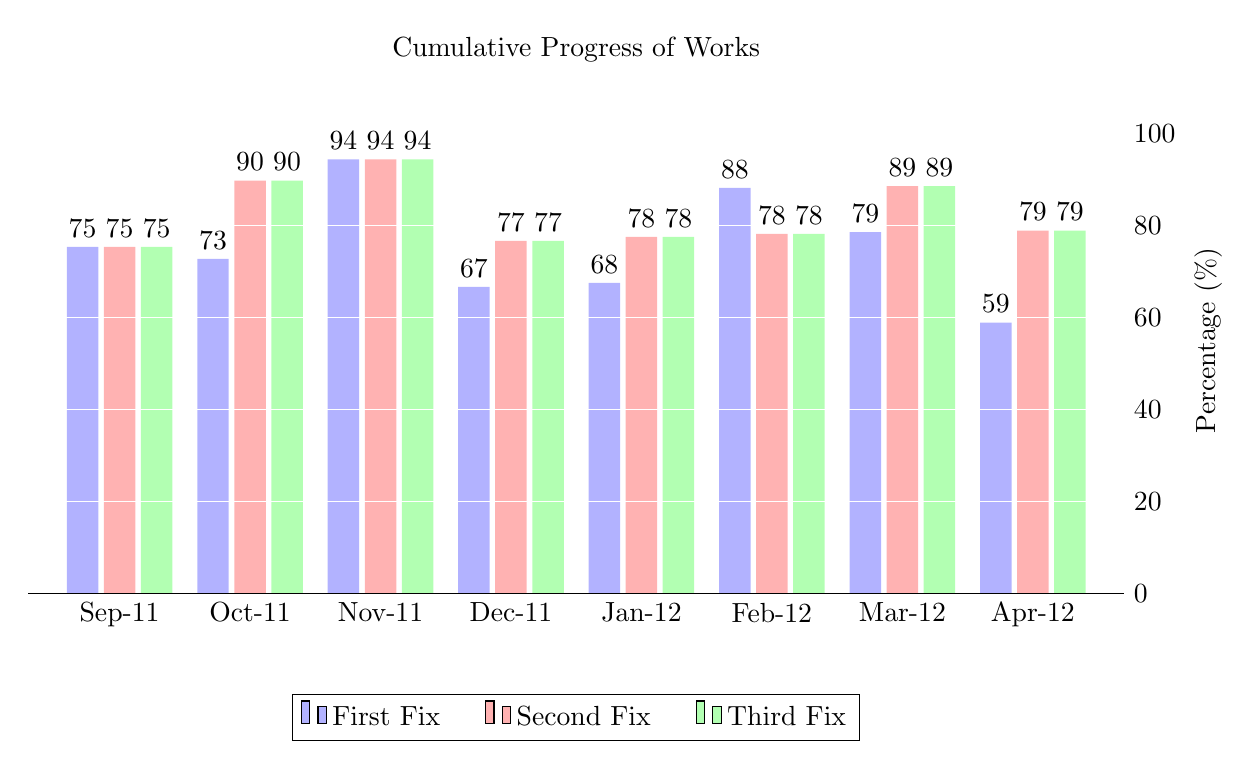
\begin{tikzpicture}
  \centering
  \begin{axis}[
        ybar, axis on top,
        title={Cumulative Progress of Works},
        height=8cm, width=15.5cm,
        bar width=0.4cm,
        ymajorgrids, tick align=inside,
        major grid style={draw=white},
        enlarge y limits={value=.1,upper},
        ymin=0, ymax=100,
        axis x line*=bottom,
        axis y line*=right,
        y axis line style={opacity=0},
        tickwidth=0pt,
        enlarge x limits=true,
        legend style={
            at={(0.5,-0.2)},
            anchor=north,
            legend columns=-1,
            /tikz/every even column/.append style={column sep=0.5cm}
        },
        ylabel={Percentage (\%)},
        symbolic x coords={
           Sep-11,Oct-11,Nov-11,Dec-11,
           Jan-12,Feb-12,
           Mar-12,
          Apr-12},
       xtick=data,
       nodes near coords={
        \pgfmathprintnumber[precision=0]{\pgfplotspointmeta}
       }
    ]
    \addplot [draw=none, fill=blue!30] coordinates {
      (Sep-11,75.4064)
      (Oct-11, 72.7961) 
      (Nov-11,94.4597)
      (Dec-11,66.6786) 
      (Jan-12,67.5600) 
      (Feb-12,88.2339)
      (Mar-12,78.6138) 
      (Apr-12,58.9129) };
   \addplot [draw=none,fill=red!30] coordinates {
      (Sep-11,75.4064)
      (Oct-11, 89.7961) 
      (Nov-11,94.4597)
      (Dec-11,76.6786) 
      (Jan-12,77.5600) 
      (Feb-12,78.2339)
      (Mar-12,88.6138) 
      (Apr-12,78.9129) };
   \addplot [draw=none, fill=green!30] coordinates {
      (Sep-11,75.4064)
      (Oct-11, 89.7961) 
      (Nov-11,94.4597)
      (Dec-11,76.6786) 
      (Jan-12,77.5600) 
      (Feb-12,78.2339)
      (Mar-12,88.6138) 
      (Apr-12,78.9129) };

    \legend{First Fix,Second Fix,Third Fix}
  \end{axis}
  \end{tikzpicture}


%%%%%%%%%%%%%%%%%%%%%%%%%%%%%%%%%%%%%%%%%%%%%%%%%%%%%%%%%%%
\end{spacing}
%%%%%%%%%%%%%%%%%%%%%%%%%%%%%%%%%%%%%%%%%%%%%%%%%%%%%%%%%%%%
%%%%%%%%%%%%%%%%%%%%%
%% FIN DU DOCUMENT %%
%%%%%%%%%%%%%%%%%%%%%
\end{document}